\documentclass[12pt,a4paper,titlepage]{article}
%\usepackage[doublespacing]{setspace}
\usepackage[utf8]{inputenc}         %This is used for ASKII digits.
\usepackage{amsmath, amssymb}       %This is for mathematic statements,check"amath.colorado.edu/documentation/LaTex/Symbols.pdf"
\usepackage{amsfonts,mathrsfs}      %fonts~~
\usepackage{graphicx}               %This is for graph inserting.
\usepackage{paralist}               %Give me compact lists!!!!! 'compactitem' 'compactenum' 'compactdesc'
%\usepackage{bm}
\usepackage{caption2}                 %various kinds of bold texts.
\usepackage[top =2.54cm, bottom =2.54cm, left =3.18cm, right =3.18 cm]{geometry}
\usepackage{indentfirst}            %Indent the first letter
\usepackage{fancyhdr}               %Below is the head of the article.
\pagestyle{fancy}
\usepackage{booktabs}
\usepackage{lastpage}
\lhead{Team \# 33131}
\rhead{Page \thepage{} of \pageref{LastPage}}
\cfoot{}
%\numberwithin{equation}{section}    %Numbering of the equations will be based on sections.
%\usepackage{amsthm}
%\theoremstyle{definition}
%\newtheorem{def}{Definition}  %Below set the theorem system.
%\theoremstyle{plain}
%\newtheorem{thm}[law]{Thm}
%\theoremstyle{remark}
%\newtheorem*{remark}{Remark}
\newcommand{\boldit}[1]{\textbf{\textit{#1}}}
\usepackage{float}
\usepackage{paralist}
\usepackage{url}

\begin{document}

\title{Human Capital Model} \date{\today{}}
\maketitle

\tableofcontents

\newpage

\section{Introduction}
\label{sec:introduction}

Considering the shortage of the talent, it's essential for companys to
retain good people and make them well-trained. However, current
situation is not satisfactory while many talents always tend to get a
good job via job-hopping, causing orgnizational churn in employees who
are closely connected to them. In order to simulate this process and
improve it, we build a human capital model based on Social Network
Analysis and Markov process.

\subsection{Restatement of the Problem}
\label{sec:restatement-of-the-problem}

Problem C describe ICM as an orginaization of 370 people on human
capital. The company is facing some issues. ICM tend to make a
positive work atmosphere to gain the loyalty of an employee in their
early time.The churn of an some employee makes effect on productivity
and emotion on other employee. Lower quality employees often stay with
the company for a full career. The churn rate is 18\% per year and
mid-level positions suffer high  churn rate, even twice the average
rate of the rest of the company. HR prefer matching employees to the
right position. It only provides promotion opportunity for those who
have several years of work experience. ICM usually has only 85\% of
its 370 positions filled at any time and HR office is actively hiring
about 8\%-10\% of the ICM positions. The CEO salary is approximately
10 times the median of the salaries of all the employees, compared to
hundreds of times the median as found in many companies.

There are several tasks we need to finish according to our model:

\begin{itemize}
\item Build a Human Capital network model of ICM organization’s
  personnel situation.

\item Identify dynamic processes within the Human Capital network,
  which includes orginizatinal churn and direct and indirect effects on
  the organization’s productivity.

\item Analyze your organization’s budget requirements over the next 2
  years.

\item Judge if ICM could sustain its 80\% full status for positions if
  the annual churn rate for all positions goes to 25\% and 35\%
  respectively. Calculate the costs of these higher turnover rates and
  describe the indirect effects of these high churn rates.

\item Simulate the impact of 30\% churn in both junior managers and
  experienced supervisors, if other churn values remain at 18\%.It
  assumes that there is no external recruiting and ICM promote only
  qualified employees for the next two years.

\item Connect our Human Capital network to other organizational
  network layers such as information flow, trust, influence, and
  friendship that the other offices of ICM are considering building.
\end{itemize}

% the main section of the paper
\section{Human Capital Model}
\label{sec:human-capital-model}

\subsection{Assumptions and Justifications}
\label{sec:assumptions-and-justifications}

\begin{itemize}
\item \textbf{assumption 1} If an employee has probability to
  promote, he won't churn.

The possibility of the unforeseen accidents, which could force an
employee to leave his position, is neglected. Based on human nature,
an employee will stay at his position to chase for higher level.

\item \textbf{assumption 2} For a vacancy,if there exists an
  employee measures up to it already, ICM won't recruit for it.

Since recruiting good people is difficult, time consuming and
expensive according to issue 5, it is wasteful to recruit for a
position if an employee can promote to it.

\item \textbf{assumption 3} Demotion won't occur.

\item \textbf{assumption 4} Administrative clerk won't promote or be
  transferred.

\item \textbf{assumption 5} Each division or office have at least one
  middle manager or senior manager.

\end{itemize}

\subsection{Model Overview}
\label{sec:model-overview}

Most research for human capital can be classified as either
microscopic and macroscopic. Since either macroscopic or microscopic
methods are difficult to solve our problem perfectly, we approach the
problem with the combination of macroscopic and microscopic methods.

To measure the ability of each person, we use Quantitative Management
Performance. Via this measurement, we can classify differient kinds of
employees which will influence the promotion process.

To build the employee network and analyze its properties, we employ
the social network analysis (SNA) technique. In our case, the
employees are viewed as nodes and relationships as links among
them. So, We can simulate the complex relationship via this network.

Definitions of symbols employed in this section are listed in Table
\ref{variable1}:
\begin{table}
  \centering
  \begin{tabular}{l p{10cm}}
  \toprule{}
  Variable & Description \\
  \midrule{}
  $i$            &Index of an employee \\
  $L_{i,t}$          &The level of $i$ \\
  $s_{ij,t}$        &The relation strength from $i$ to $j$ \\
  $a_{ij,t}$        &Represent the influence caused by relationship
                    between superior and subordinate \\
  $f_{ij,t}$        &Represent the influence caused by relationship
                    between person with many friends and person with
                    few friends \\
  $c_{i,t}$        &Clustering Coefficient of $i$ \\ \bottomrule{}
\end{tabular}
\caption{Variables and Descriptions}\label{variable1}
\end{table}

\subsection{Human Performance Model}
\label{sec:human-model}

In this part, we buid a people model to evaluate an employee in four
aspects, in terms of \textbf{Quantitative Management Performance} ---
work achievement, work ability, work attitude and potential. These
four aspects are supposed to be quantized according to annual
evaluation based on performance as judged by the supervisor and we
take these independent variables as $A_{ac_i}$, $A_{ab_i}$, $A_{at_i}$
and $A_{po_i}$ for each employee $i$. For each of the four parameters,
it goes from 0 to 1. The statues are used for calculating the
probability that employee can promote. Meanwhile, they influence
leaving probability and team cohesiveness as well.

It is obvious that some of the parameters are somehow more important
than others. So in an effort to make our model more accurate and
reliable,we introduce a weighted index of deviation $AD_i$, with
\begin{equation}
  A_i=w_{ac} \cdot A_{ac_i} + w_{ab} \cdot A_{ab_i} + w_{at} \cdot A_{at_i} +
  w_{po} \cdot A_{po_i}
\end{equation}

We determine weights via the Analytical Hierarchy Process(AHP) [Saaty
1982]. We build a $4 \times 4$ reciprocal matrix by pair comparison:
\begin{center}
\begin{tabular}{|c|c|c|c|c|}
\hline
       &$A_{ac}$      &$A_{ab}$  &$A_{at}$    &$A_{po}$  \\ \hline
 $A_{ac}$ & 1           & 5 & 2            &1            \\ \hline
 $A_{ab}$ &$\frac{1}{5}$ & 1 &$\frac{1}{3}$ & $\frac{1}{4}$\\ \hline
 $A_{at}$ &$\frac{1}{2}$ & 3 & 1            &1            \\ \hline
 $A_{po}$ &1            & 4 & 1            &1            \\ \hline
\end{tabular}
\end{center}

The meaning of the number in each cell is explained in Figure
\ref{important}. The numbers themselves are based on our own
subjective decisions.

\begin{table}[htb]
  \centering
  \begin{tabular}{cl}
    \toprule{}
    Intensity of Importance&Definition \\ \midrule{}
    1                      &Equal Importance \\
    2                      &Weak or slight \\
    3                      &Moderate importance \\
    4                      &Moderate plus \\
    5                      &Strong importance \\
    6                      &Strong plus \\
    7                      &Very strong or demonstrated importance \\
    8                      &Very, Very strong \\
    9                      &Extreme importance \\ \bottomrule{}
  \end{tabular}
  \caption{The fundamental scale of absolute numbers}\label{important}
\end{table}

We then get the weight of each factor by calculating the bigest
eigenvalue and it's corresponding eigenvector, as given in Table \ref{weight}.

\begin{table}
\begin{center}
\begin{tabular}{ccccc} \toprule{}
  Factor  &$A_{ac}$    &$A_{ab}$   &$A_{at}$    &$A_{po}$\\ \midrule{}
  Weight  &0.3805  &0.0709  &0.2371  &0.3030\\ \bottomrule{}
\end{tabular}
\end{center}
\caption{Weight for factors}\label{weight}
\end{table}

We test the consistency of the preferences for this instance of the
AHP.\@ For good consistency [Alonso and Lamata 2006, 446 - 447]:

\begin{itemize}
\item The principal eigenvalue $\lambda_{max}$ of the matrix should be
  close to the number n of alternatives, here 4; we get $\lambda_{max} = 4.047$.
\item The consistency index $CI = (\lambda_{max}-n)/(n-1)$ should be close to 0; we get $CI = 0.0157$.
\item The consistency ratio $CR = CI/RI$ (where RI is the average
  value of CI for random matrices) should be less than 0.1; we get $CR
  = 0.0182$.
\end{itemize}

Hence, our decision method displays perfectly acceptable consistency
and the weights are reasonable.

\subsection{Social Network Model}
\label{sec:social-network-model}

The social network model contains a directed weighted graph $G(V,E)$
in which $V$ denote the employees and $E$ denote the connection
between employees. Since there are personnel changes, $G(V,E)$ will
change with time goes by. In order to simulate this situation, we use
$G_t(V_t,E_t)$ instead of $G(V,E)$ where $t$ is a discrete
variable. So $G_t(V_t,E_t)$ denote the social network in the $t$-th
month.

First, we explain the way we build edges of $G_t(V_t,E_t)$.

When $t = 0$, there are about $370 \times 85\%$ nodes (employees) in
$G_t$. We build edges between employees in the same division or
office, since employees in the same division or office certainly know
each other. So each division or office form a complete graph and
employees in the differient division or office don't know others,
which is impossible. To solve this problem, we build 10 edges for each
employee with employees in other divisions with equal
probability. Then we build the other edges with probability
$p = \frac{\left|N_{i,t} \cap N_{j,t}\right|}{\left|N_{i,t} \cup
    N_{j,t}\right|}$
which is called Jaccard similarity coefficient[Jaccard 1901].

When $t > 0$, there will be employees leaving or joining the
company. If an employee leave, all his edges with other employees with
be deleted. If an employee newly join the company, he will follow
steps which employees at $t = 0$ take. This is the dynamic process of
graph $G_t(V_t,E_t)$.

Let $s_{ij,t}$ denote the weight from $i$ to $j$ at time $t$. We have
these properties of $G_t(V_t,E_t)$:

\begin{itemize}
\item $s_{ij,t} \ne s_{ij,t}$

  We made this graph directed and weighted because one person may
  consider another person his best friend while that person doesn't
  consider him a good friend. This situation may appear because of the
  relationship between superior and subordinate and the relationship
  between person with more friend and person with less friend. In
  general, $s_{ij,t} \ne s_{ij,t}$ for the reason above.

\item $s_{ij,t}=\dfrac{a_{ij,t}+f_{ij,t}}{2}$

  $a_{ij,t}$ denote the influence caused by the relationship between
  superior and subordinate, $f_{ij,t}$ denote the influence caused by
  the amount of friends for $i$ and $j$. We define
$$a_{ij,t}=\begin{cases}
  \frac{1}{2+\left|L_{i,t}-L_{j,t}\right|}, & L_{i,t} \ge L_{j,t} \\
  1-\frac{1}{2+\left|L_{i,t}-L_{j,t}\right|}, & L_{i,t} < L_{j,t} \\
\end{cases}$$
, where $L_{i,t}$ denote the level of $i$ at time $t$, and
$$f_{ij,t}=\frac{\left|N_{i,t} \cap
    N_{j,t}\right|}{\left|N_{i,t}\right|}$$.

\end{itemize}

\subsection{Promote and Churn Model}
\label{sec:promote-and-churn-model}

First, we explain the model of promotion aimed to predict the
promotion probability. We define the promotion rate of $i$ as
$p_i$ to evaluate the probability to promote. As a matter of fact, if
there is a vacancy, judging if an employee suits the site involves
work experience and ability. It is essential that he is supposed to
have several years of work experience according to issue 6. If an
employee satisfies the experience condition, it turns out to think
about his ability. Since in Human Performance Model, each employee's
ability is evaluated by a parameter $A_{D_i}$. For each level of
position, it has an ability standard, as shows in Table[]. The ability
of an employee are supposed to reach the four standard parameters
respectively, otherwise its $p_i$ is 0. For those who reach the
standard, the promotion probability can be calculated by the equation:
$p_i =\dfrac{A_{D_i}}{\sum_{\alpha} A_{D_\alpha}}$ where $\alpha$ represent
employee who have probability to promote.

According to assumption 1 and assumption 2, from $t$ to $t+1$, the
model update once according to the following rules:

\begin{itemize}
\item [\textit{step 1}] Promotion: If there's a vacancy in superior
  and $i$ has the ability to occupy this position, let $L_{i+1,t} =
  L_{i,t}+1$ with probability mentioned above and build edges between
  $i$ and his new colleagues.
\item [\textit{step 2}] Churn: If $i$ isn't promoted, he will have the
  probability to churn with a churn rate $l$.
\item [\textit{step 3}] Stay: If $i$ hasn't been promoted or churned,
  he will keep his job and do nothing.
\item [\textit{step 4}] Recruit: Recruit for vacancies when all the
  employees have done these 3 steps above.
\end{itemize}

\section{The Improved Model}
\label{sec:the-improved-model}

\subsection{Assumptions and Justifications}

\begin{itemize}
\item \textbf{assumption 1} For the promotion probability and
  organization change, the other factors effects the churn probability
  is invariable.

Though churn derives from varieties of reasons and they are actually
lacking of known conditions and data to estimate them, we have to
regard it as stable in our model.
\end{itemize}

\subsection{Organizational Churn}

The network of the company we've built changes in terms of
orgnizational churn and promotion. Considering various of factors in
reality, we build an orgnizational churn and promotion model to
predict the dynamic process.

The first part of the model is churn model.We define the churn rate of
an employee $i$ as $l_i$ to evaluate the probability to churn. $l_i$ is
usually controlled by sorts of factors to different degrees. We
divides $l_i$ into three parts:$l_{i1}$, $l_{i2}$ and$l_{i3}$.  $l_{i1}$
represents the churn rate because of lacking of promotion
opportunity. $l_{i2}$ represents the churn rate because of the changes
of other employees related to employee $i$. To simplify our model, we
presume that $l_i1$, $l_i2$ is linear correlated with $(1-p_i)$ and
$s_i$, which means

\begin{equation}
  l_{i1}=\lambda_1(1-p_i),l_{i2}=\lambda_2s_i
\end{equation}

$\lambda_1$ and $\lambda_2$ could be ensured in later calculation.

$l_{i3}$ represents the other factors we can't get any information from
the known conditons so that we regard it as stable.  Thus

\begin{equation}
  l_i = \lambda_1(1-p_i) + \lambda_2s_i +l_i3
\end{equation}

After analyzing a great deal of churn rate reports, we get the
composition of the three parts are 10.9\%, 2.2\% and 75.4\%
respectively. According to the percentage and the general
churn rate 18\%, we can calculate $\lambda_1$, $\lambda_2$ and
$l_{i3}$. As an orinigal condition,it satisfies

\begin{equation}
\label{lambda}
\begin{cases}
  \lambda_1 \sum_{i=1}^{370}(1-p_i) & =10.9\% \times 370 \times 1.5\% \\
  \lambda_2 \sum_{i=1}^{370}s_i & =2.2\% \times 370 \times 1.5\% \\
  l_{i3} & =1.5 \% \times 75.4 \%
\end{cases}
\end{equation}

Thus we can use Equation\ref{lambda} to calculate the churn rate $l_i$.

Analyzing the consequence of this phenomenon, we use our program to
simulate this process. As a result, we find a organizational churn in
our simulation as shown in Figure \ref{organizational-churn}.

\begin{figure}[htb]
  \centering
  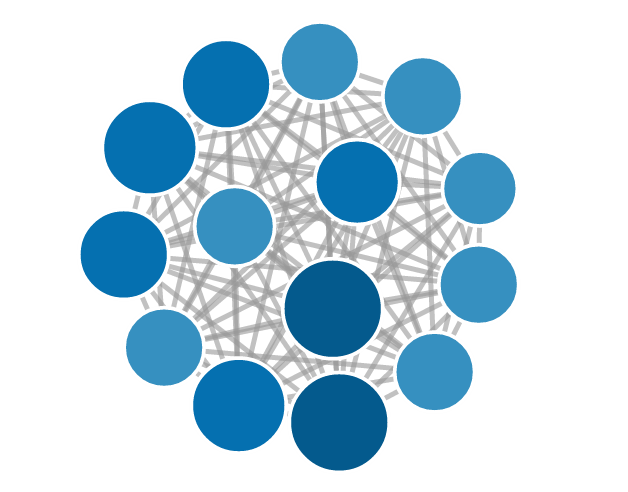
\includegraphics[width=4cm]{Pic3_0.png}
  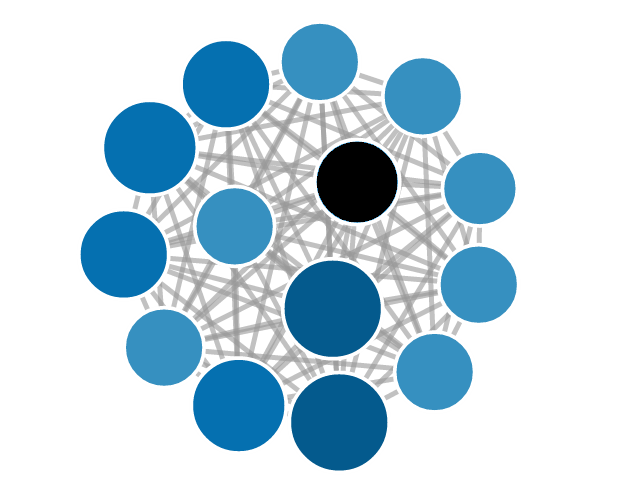
\includegraphics[width=4cm]{Pic3_1.png}
  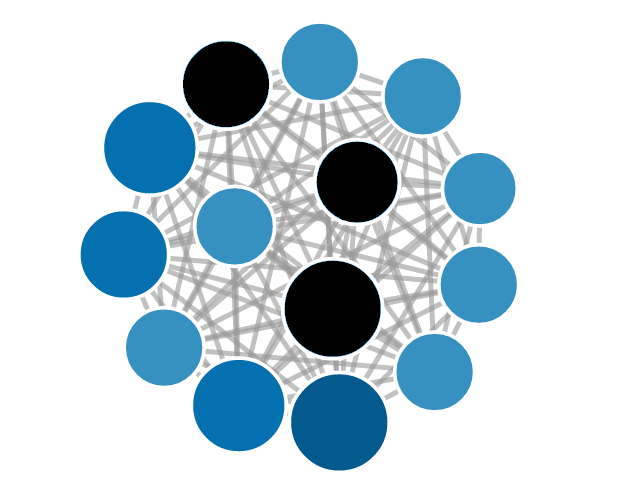
\includegraphics[width=4cm]{Pic3_2.png}
  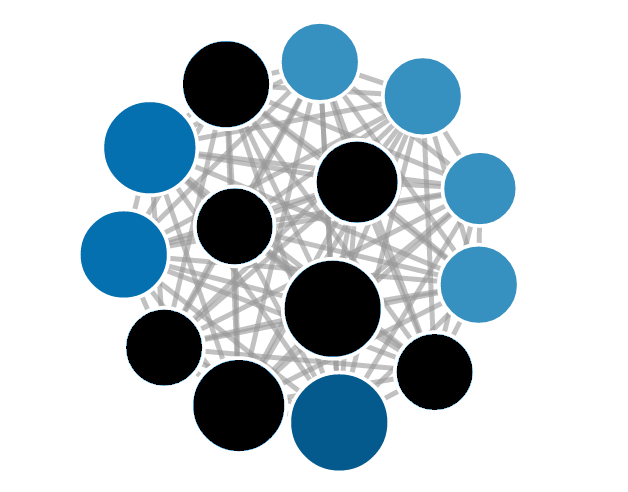
\includegraphics[width=4cm]{Pic3_3.png}
  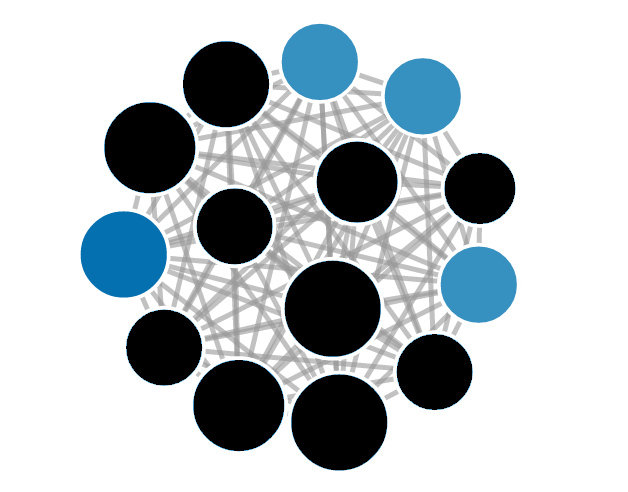
\includegraphics[width=4cm]{Pic3_4.png}
  \caption{Organizational Churn}\label{organizational-churn}
\end{figure}

The black spots in the graph denote employees who have churned

\subsection{Productivity}

First, we explain the concept of clustering coefficient [Duncan
J. Watts and Steven Strogatz 1998] of $i$ denoted as $c_{i,t}$, which
is a measure of the degree to which nodes in a graph tend to cluster
together. $c_{i,t}$ is defined as:

$$c_{i,t}=\dfrac{\left| \left\{ s_{jk,t}:v_j,v_k \in M_i,s_{jk,t} \in E
    \right\} \right|}{k_{i,t}(k_{i,t}-1)}$$
where
$M_{i,t}=\left\{ v_j:s_{ij,t} \in E \and s_{ji,t} \in E \right\}$ and
$k_{i,t}=\left| N_{i,t} \right|$.


\section{Performance and Analysis}
\label{sec:performance-and-analysis}

\subsection{Analysis for Task 3}
\label{sec:analysis-for-task-3}

We assume that the company offers training programs for its employees monthly and newly hired employees start to get their salaries next month after they enter the company. With these two assumption, results can be drawn according to our model through simulation.

Budget can be divided into threee parts: salary budget, training budget and recruiting budget. The budget requirement predicted for next two years is listed in the table below in terms of $\sigma$.

\begin{tabular}{*{4}{c}}\toprule[2pt]
Total Budget & Salary Budget & Training Budget & Recruiting Budget\\ \midrule
1170.8$\sigma$ & 951.387$\sigma$ & 164.423$\sigma$ & 55.08$\sigma$ \\ \bottomrule[2pt]
\end{tabular}

\subsection{Analysis for Task 4}
\label{sec:analysis-for-task-4}


\begin{figure}[htb]
  \centering
  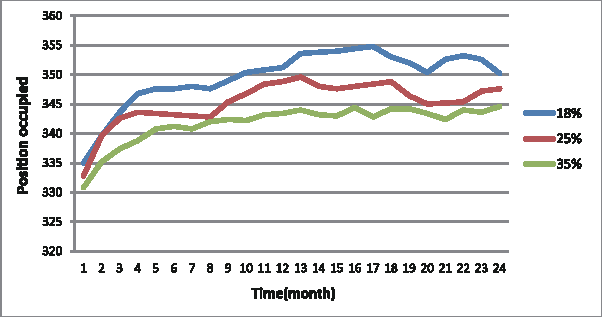
\includegraphics[width=10cm]{task4_p.pdf}\\
  \caption{Status of positions}\label{t4_p}
\end{figure}

To analyze the status of positions under different churn rate, we use
our model to simulate dynamic processes with these churn rate
constraints. We execute our program 100 times for each churn rate and
average the predicted values. Figure \ref{t4_p} shows the averaged
results our model predicted. Under all of these three conditions, the
number of employees in the company keeps rising. The higher the churn
rate, the lower the final full rate the company reaches after two
years. But ICM can sustain its 80\% for positions even if the churn
rate goes to 35\% according to our model's precition.

\begin{figure}[htb]
  \centering
  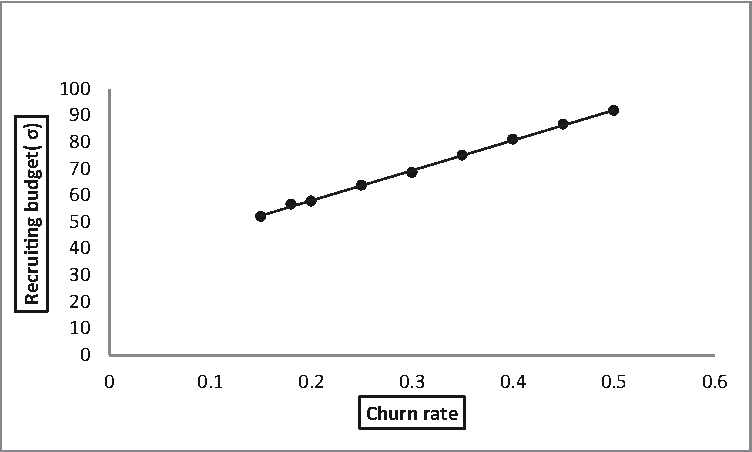
\includegraphics[width=10cm]{task4_r.pdf}\\
  \caption{Recruiting budget}\label{t4_r}
\end{figure}
\begin{figure}[htb]
  \centering
  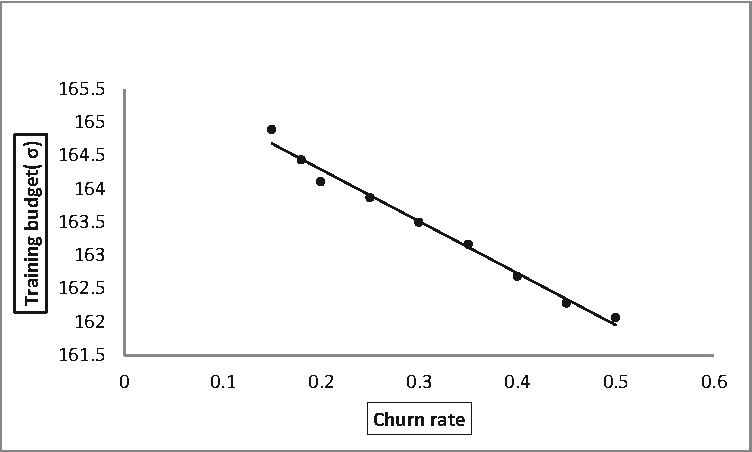
\includegraphics[width=7cm]{task4_t.pdf}
  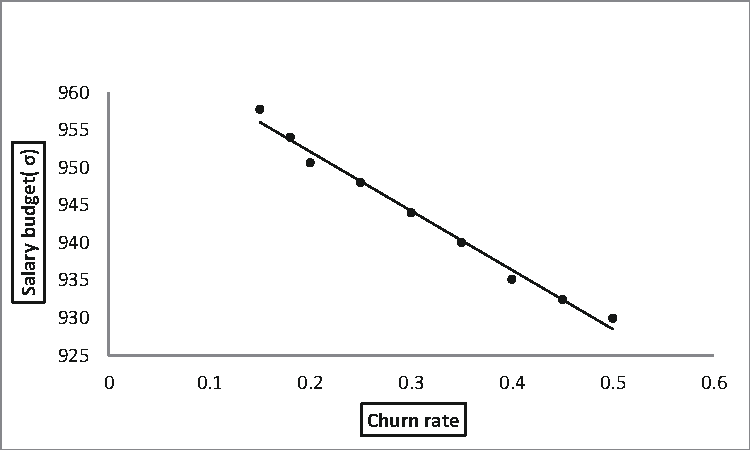
\includegraphics[width=7cm]{task4_s.pdf}\\
  \caption{Training budget and salary budget}\label{t4_t_s}
\end{figure}
The churn rate effect the budget of the company as well. The three
parts of the bugdet behave differently when churn rate increases. The
calculated budget is shown in Figure \ref{t4_r} and Figure
\ref{t4_t_s}. Each data point in three charts is an averaged result of
10 predictions and a linear trendline is added to each chart. It is
clear that recruiting budget showed in Figure \ref{t4_r} is likely to
be proportional to the churn rate while salary budget and training
budget showed in Figure \ref{t4_t_s} are likely to be inversely
proportional to the churn rate.

To maintain enough employees, the company has to spend more on
recruiting. So high turnover rate directly increase the recruiting
budget. High turnover rate's effect on training budget and salary
budget is more complex. On the one hand, when churn rate goes up,
vacancies in the middle level keeps rising due to long recruiting time
and low promote rate. On the other hand, the vacancies in lower level
remains low because of the short recruiting time. So the full rate of
the company decreases when churn rate rises. Since training budget and
salary budget are closely related to full rate, both of them decrease
when turnover rate goes up.

\subsection{Analysis for Task 5}
\label{sec:analysis-for-task-5}

\begin{figure}[htb]
  \centering
  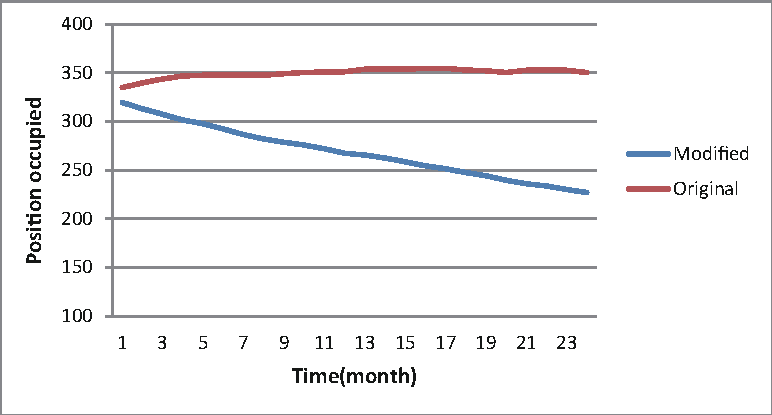
\includegraphics[width=10cm]{task5_p.pdf}\\
  \caption{Status of position}\label{t5_p}
\end{figure}
We apply following changes to our model to simulate the required process:\\
\begin{itemize}
\item Change the churn rate of junior managers and experienced supervisors to 30\%
\item Prohit external recruiting
\item Promoting only qualified employees
\end{itemize}
\begin{table}
        \begin{center}
                \begin{tabular}{l|cc}\toprule[2pt]
                \bfseries Level of Position & \bfseries Modified & \bfseries Original\\ \midrule
                Senior manager/Executive & 5.6 & 8.4\\
                Junior manager/Executive & 9.0 & 18.4\\
                Experienced supervisor & 7.4 & 23.0\\
                Inexperienced supervisor & 9.2 & 23.2\\
                Experienced employee & 72.6 & 107.4\\
                Inexperienced employee & 99.6 & 149.6\\
                Administrative clerk & 24.0 & 24.0\\ \bottomrule[2pt]
                \end{tabular}
                \caption{Status of position}\label{t5_p_t}
        \end{center}
\end{table}

The result of simulation is shown in Figure \ref{t5_p} and Table
\ref{t5_p_t}. All the data shown is an average of ten
predictions. While the number of positions occupied remains stable
with origial conditions, it drops remarkably with modified
conditions.

We list specific data of each level in Table \ref{t5_p_t}. In the
modified case, the numbers of employees are lower than original case
especially the those of middle levels. Since there is no external
recruiting in modified case, it is obivious that the full rate will
decrease due to employees' leave. Although some qualified employees
can be promoted into higher level, the high churn rate of the middle
level and difficulty of satisfying the promotion conditions make the
numbers of middle level employees relatively low. The situation given
in that task 5 will cause unrecoverable damage to ICM's HR
health. With the full rate of middle level employees lower than 50\%,
the HR structure is broken into fragments and the company won't be
able to function normally.


\section{Advice for HR}
\label{sec:advice-for-hr}

As the HR manager faces many problems such as identifying those that
are likely to churn and maximizing employees' knowledge and
abilities, we explain our further improved model.

\subsection{Incentive Mechanism}
\label{sec:incentive-machanism}

A worker is more likely to churn if he or she was connected to other
former employees who have churned. So there are two kinds of people
who should be highly paid attention to and incented.

First, we should pay attention to those who have more friends than
others. Because of their wide connection with other employees, the
consequence of their churn may be destructive, which cause many
friends' churn.

Second, we focus on those having more friends who have churned
during the past year. This kind of people have a great probability to
churn because of the influence of others.

We choose one sample in our simulations and 50 people in this sample
to explain our incentive mechanism.

\begin{figure}[htb]
  \centering
  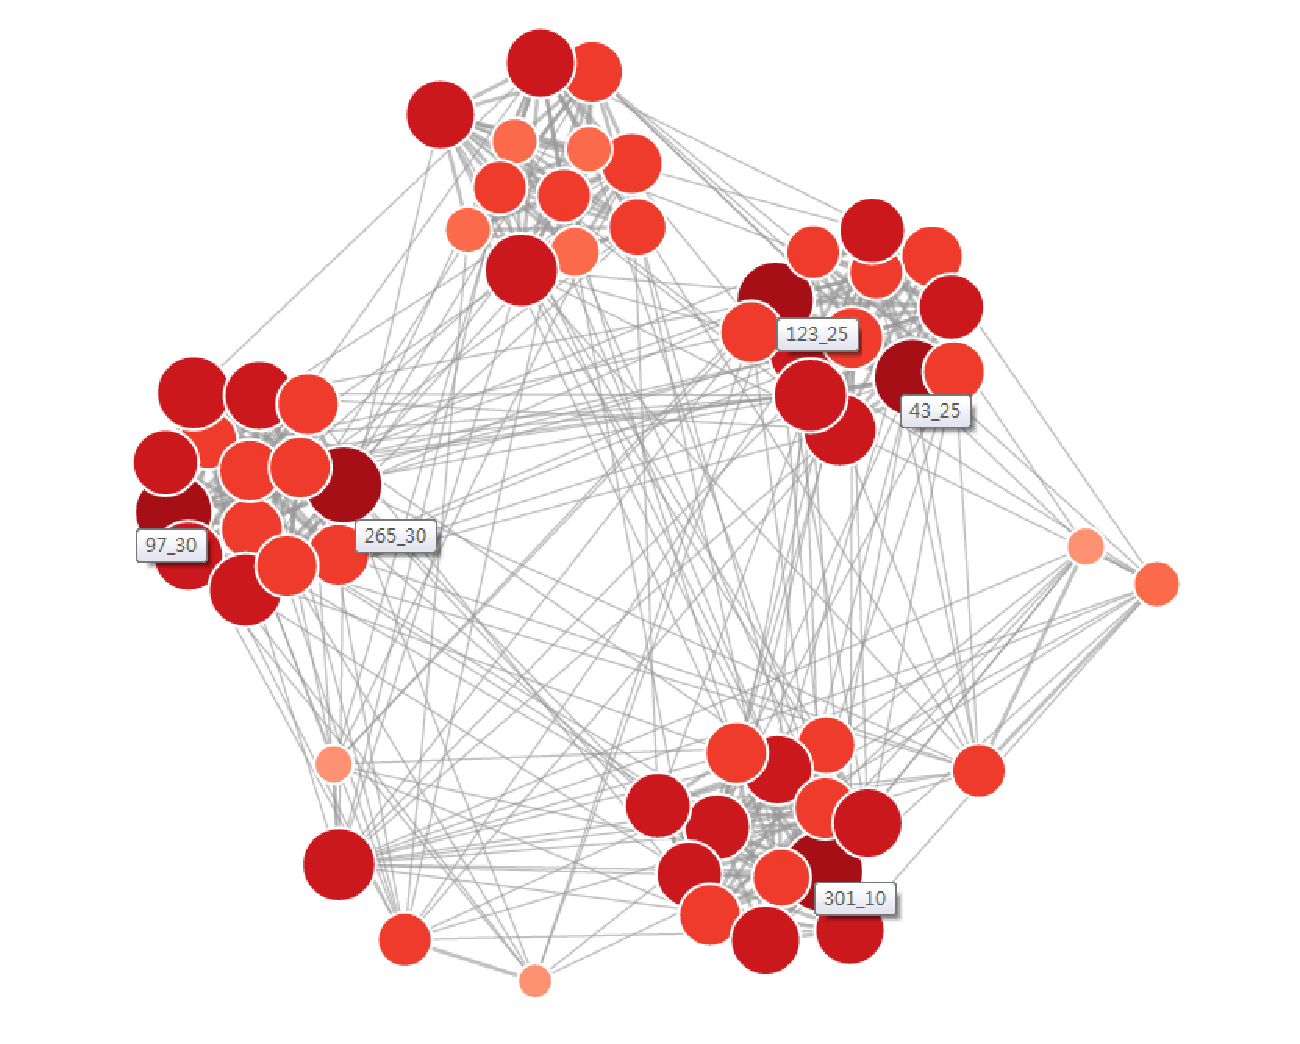
\includegraphics[width=7cm]{p1.eps}
  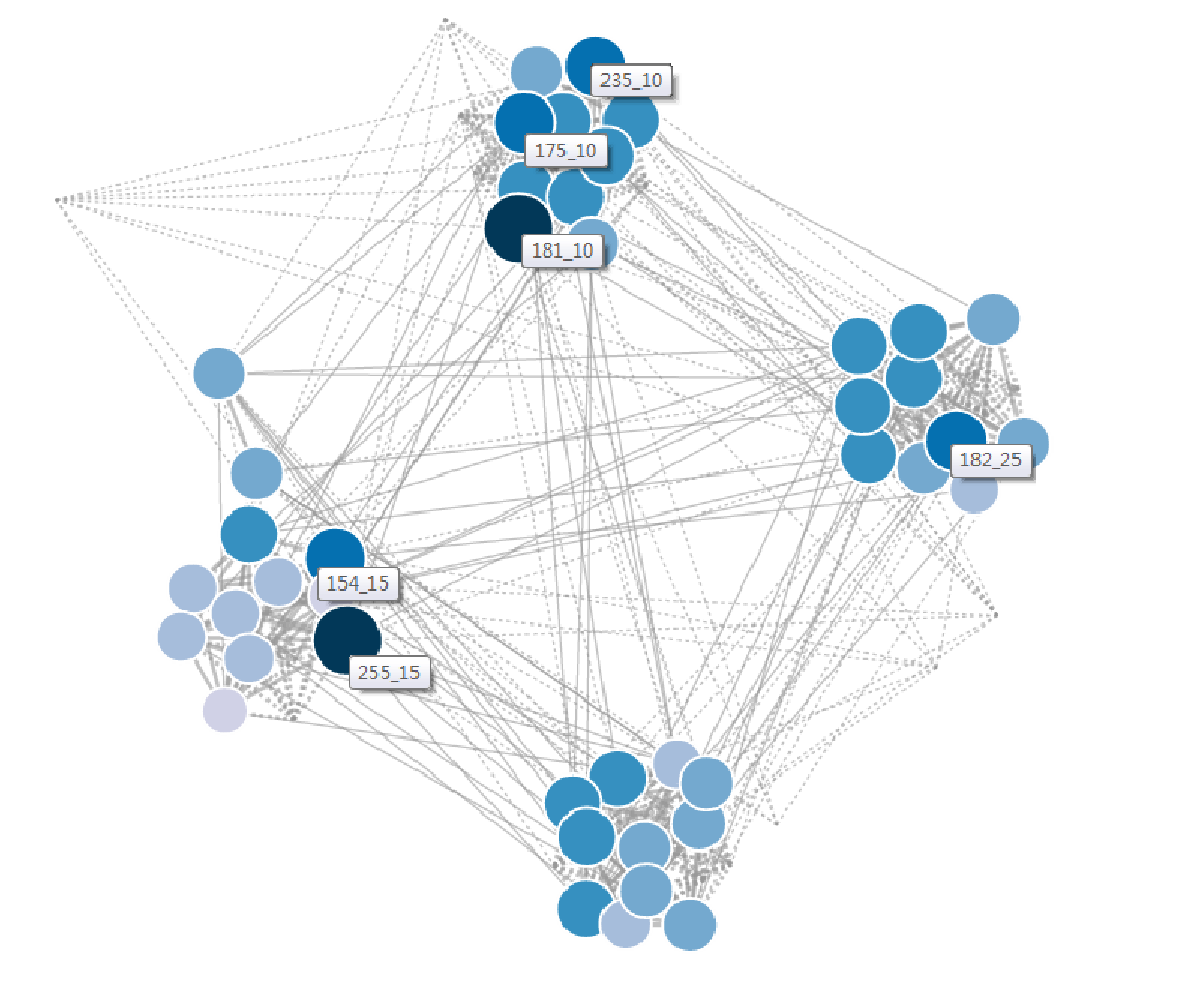
\includegraphics[width=7cm]{p2.eps}
  \caption{employees should be pay attention
    to}\label{incentive-mechanism}
\end{figure}

In Figure\ref{incentive-mechanism}, as we can see, each vertex
represents an employee, each full line represents a relation between 2
employees, each imaginary line represent an relation between person
who is on the job and person who churn. There are 5
employees in left graph we should pay attention to which are
43, 97, 123, 265 and 301 because they have more full lines than
others. There are 6 employees in the right graph we should pay
attention to which are 154, 175, 181, 182, 235 and 255 because they
have more imaginary lines than others.

We provide incentives to these employees which will decrease their
probabilities to churn.

At time $t$, we choose top 10\% of the employees which have the
properties above and decrease their churn rate by 50\%. As shown in
Figure\ref{churn-rate}, the churn rate decrease rapidly.

\begin{figure}[htb]
  \centering
 % \includegraphics[width=11cm]{p4.pdf}
  \caption{Churn rate-Time Curve}
  \label{churn-rate}
\end{figure}

\subsection{Matching Employees to the Right Position}
\label{sec:matching-employees-to-the-right-position}

We consider different abilities of different employees. As we have an
annual evaluation based on performance for each employee and each
division or office has it's necessarily needed abilities, we can match
employees with their most suitable position.

Because the evaluation is given annually, we reassign employees
annually according to their abilities and the formula below:

\begin{equation}
m_{i,j} =
{(A_{ac_i}-B_{ac_j})}^2 + {(A_{ab_i}-B_{ab_j})}^2 + {(A_{at_i}-B_{at_j})}^2
+ {(A_{po_i}-B_{po_j})}^2
\end{equation}

where $B_{ac_j}$, $B_{ab_j}$, $B_{at_j}$, $B_{po_j}$ represent the
abilities needed for position $j$.

Defining $x_{ij}=\begin{cases} 1 , & \mbox{reassign employee } i
  \mbox{ to position } j \\ 0,&\mbox{otherwise} \end{cases}$, we can
describe this problem as a mathematical programming problem:

\begin{equation}
  \begin{split}
  \min&\sum_{i=1}^n\sum_{j=1}^m m_{ij}x_{ij} \\
  s.t.& \sum_{j=1}^m x_{ij}=1, i=1,2,\ldots,n \\
  &\sum_{i=1}^n x_{ij} \le1,j=1,2,\ldots,m \\
  &x_{ij}=0 \mbox{ or } 1,i=1,2,\ldots,n,j=1,2,\ldots,m
  \end{split}
\end{equation}

We can solve this problem via Kuhn–Munkres algorithm [Harold Kuhn and
James Munkres 1957] whose time complexity is $O(n^4)$.

We reassign them once a year according to their
evaluation. Figure\ref{reassign} shows productivity with reassignment
and without reassignment. We can find that the productivity increase
rapidly after reassign employees, which means reassignment truly help
with productivity of the company.

\begin{figure}[htb]
  \centering
  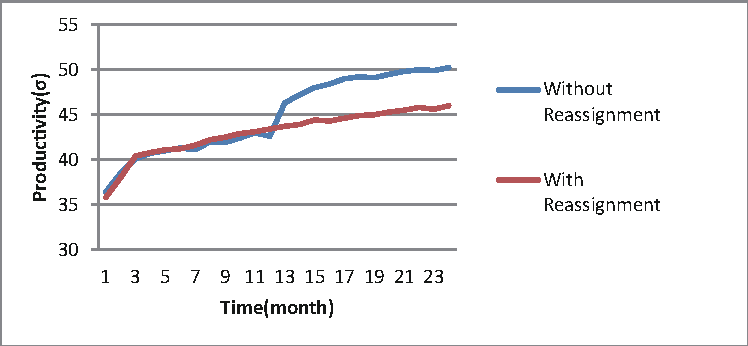
\includegraphics[width=11cm]{p3.pdf}
  \caption{Productivity-Time Curve}\label{reassign}
\end{figure}

\section{Team Science}
\label{sec:team-science}

This part shows how our model connects to other organizational network
layers such as information flow, trust, influence, and
friendship. Number the layers from 0 to
k. $$G^\alpha=(V^\alpha,E^\alpha), \alpha=1,2,\ldots,k$$ Each
$E^\alpha$ is colored by a specific color. $G^0$ reprensents the
network we built before, $G^1, G^2, \ldots ,G^k$ represent the other layers added.

Still, in each network layer $G_\alpha$, $N_i$ represents emploee
$i$. The edge $e_{ij}$ connects between two nodes $N_i$ and
$N_j$. Each edge has a value $w_{ij}^\alpha$ proving the weight of
edge $e_{ij}^\alpha$, positive correlated to the strength of
connection between two employees in network layers $\alpha$. Then we
connect these network layers together to built a general network
$G_e=(V, E, C)$, V is node set, C is color set, $E \subset  V\times
V\times C$ is edge set. In the general model, different layers effects
each other. Take for example, if the friendship between employee $i$
and employee $j$ is deeper, with other conditions the same,their
information flow is more fluent. $w_{ij}^\alpha$ is changing with time
flows and $G_e$ is a dynamic network.

However, human capital network make the maily effect on other network
layers. In the general network, if an empolyee churns or is
reassigned, the edge related to him will change. That is,
$w_{ij}^\alpha$ get a new value for all $\alpha$. Hence, human capital
network takes the lead in this effort.

\section{Sensitivity Analysis}
\label{sec:sensitivity-analysis}

a

\section{Strengths and Weaknesses}
\label{sec:strengths-and-weaknesses}

\subsection*{Strengths}
\label{sec:strengths}

\begin{itemize}
\item Our model make fully use of the theory of multilayer networks so
  that it quantizes the relation accurately and reasonablly.
\item Our model exellently proves the interaction among these
  factors:leave probability, promotion probability and productivity.
\item The network we built include both microcosmic part and
  macrocosmic part, and they react to each other.
\item Our model proves the effection of time.
\end{itemize}

\subsection*{Weaknesses}
\label{sec:weaknesses}

\begin{itemize}
\item Limited by the time,we neglected sorts of factors which are not so significant.In fact, the model still has space to be perfected.
\item The result has some randomness.
\end{itemize}

\section{Conclusions}
\label{sec:conclusions}

a

% the reference
\begin{thebibliography}{99}

\bibitem{} Huang Y. A Study of the Performance Assessment of State-owned Power Enterprisees[D]. Tianjing University, 2010.

\bibitem{} Journal T E D O T. The Investigation Report of the Condition of employee churn in 2011[J]. China New Time, 2012(2).

\bibitem{} Zhang J. The Empirical Research of the Factors effecting employee churn in Resource-oriented Enterprise in Yuncheng,Shandong [D]. Southerneast University, 2014.

\bibitem{} MEJNewman. The Structure and Function of Complex Networks[D]. University of Michigan, 2003.

\bibitem{} Fang J, Zheng Z, Bi Q, etal. A Brand-new
  Interdisciplinary Science: Network Science (Part One)[J]. Progress in Physics, 2007, 27(3).

\bibitem{} Fang J, Zheng Z, Bi Q, etal. A Brand-new
  Interdisciplinary Science: Network Science (Part Two)[J]. Progress in Physics, 2007, 27(4).

\end{thebibliography}

\label{LastPage}

\end{document}

%%% Local Variables:
%%% mode: latex
%%% TeX-master: t
%%% End:
